\shorthandon{"}
\section{Методы "встреча посередине"\ и "разделяй и властвуй".}
\shorthandon{"}

\task{Найти минимальную среднюю трудоёмкость нахождения ключа в следующей схеме шифрования, длина ключа ГОСТ = 256 бит. Сравнить с МПП.

\medskip

\begin{tikzpicture}[>=latex]
{\centering
\draw[thick, ->] (0,0) -- node[above left] {$x$} (1,0);
\draw (1,-0.5) rectangle node[midway] {$DES(k_1)$} (3.5,0.5);
\draw[thick, ->] (3.5,0) -- (4.5,0);
\draw (4.5,-0.5) rectangle node[midway] {$ГОСТ(k_2)$} (7,0.5);
\draw[thick, ->] (7,0) -- node[above right] {$y$} (8,0);
}
\end{tikzpicture}
}

\shorthandon{"}
Средняя трудоёмкость метода "встречи посередине":
$$(|K_1| + |K_2|)(1 + \ln(|K_1| + |K_2|)) = (2^{56} + 2^{256})(1 + \ln(2^{56} + 2^{256})) \approx 10 ^ {79.47}$$

\noindent Средняя трудоёмкость полного перебора: $\frac{|K_1||K_2|}{2} = \frac{2^{56} \cdot 2^{256}}{2} = 2^{311} \approx~10 ^ {93.62}$

Метод "встречи посередине"\ оказывается на 14 порядков эффективнее МПП.

Если предположить, что у нас имеется эффективный критерий, отбраковывающий ключи из $K_1$, то можно воспользоваться методом "разделяй и властвуй"\,, средняя трудоёмкость которого равна $\frac{|K_1| + |K_1|}{2} = \\ = 2^{55} + 2^{255} \approx 10 ^ {76.76}$. Этот метод ещё эффективнее в 1000 раз.

\task{Ключом являются начальные заполнения ЛРС в алгоритме получения $\gamma$ для шифра гаммирования. Предполагается, что имеется необходимое количество пар $(x, y)$. Оценить сложность нахождения ключа с помощью метода "встречи посередине"\ и сравнить с МПП.
\shorthandon{"}

\medskip

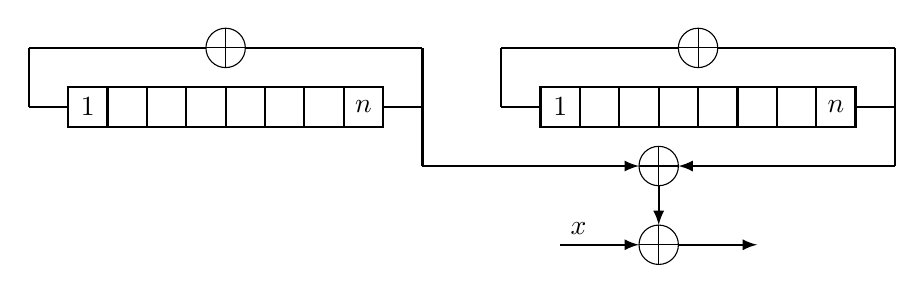
\begin{tikzpicture}[>=latex]
{\centering
\draw[thick] (0, 0) rectangle node[midway] {$1$} (0.5,0.5);
\draw[thick] (0.5, 0) rectangle (1,0.5);
\draw[thick] (1, 0) rectangle (1.5,0.5);
\draw[thick] (1.5, 0) rectangle (2,0.5);
\draw[thick] (2, 0) rectangle (2.5,0.5);
\draw[thick] (2.5, 0) rectangle (3,0.5);
\draw[thick] (3, 0) rectangle (3.5,0.5);
\draw[thick] (3.5, 0) rectangle node[midway] {$n$} (4,0.5);

\draw[thick, -] (0,0.25) -- (-0.5,0.25);
\draw[thick, -] (-0.5,0.25) -- (-0.5,1);
\draw[thick, -] (-0.5,1) -- (1.75,1);

\draw (2, 1) circle (0.25);
\draw[-] (2, 1.25) -- (2, 0.75);
\draw[-] (1.75, 1) -- (2.25, 1);

\draw[thick, -] (4,0.25) -- (4.5,0.25);
\draw[thick, -] (4.5,-0.5) -- (4.5,1);
\draw[thick, -] (2.25,1) -- (4.5,1);

\draw[thick] (6, 0) rectangle node[midway] {$1$} (6.5,0.5);
\draw[thick] (6.5, 0) rectangle (7,0.5);
\draw[thick] (7, 0) rectangle (7.5,0.5);
\draw[thick] (7.5, 0) rectangle (8,0.5);
\draw[thick] (8, 0) rectangle (8.5,0.5);
\draw[thick] (8.5, 0) rectangle (9,0.5);
\draw[thick] (9, 0) rectangle (9.5,0.5);
\draw[thick] (9.5, 0) rectangle node[midway] {$n$} (10,0.5);

\draw[thick, -] (6,0.25) -- (5.5,0.25);
\draw[thick, -] (5.5,0.25) -- (5.5,1);
\draw[thick, -] (5.5,1) -- (7.75,1);

\draw (8, 1) circle (0.25);
\draw[-] (8, 1.25) -- (8, 0.75);
\draw[-] (7.75, 1) -- (8.25, 1);

\draw[thick, -] (10,0.25) -- (10.5,0.25);
\draw[thick, -] (10.5,-0.5) -- (10.5,1);
\draw[thick, -] (8.25,1) -- (10.5,1);

\draw (7.5, -0.5) circle (0.25);
\draw[-] (7.5, -0.25) -- (7.5, -0.75);
\draw[-] (7.25, -0.5) -- (7.75, -0.5);

\draw[thick, ->] (4.5, -0.5) -- (7.25, -0.5);
\draw[thick, <-] (7.75, -0.5) -- (10.5, -0.5);
\draw[thick, ->] (7.5, -0.75) -- (7.5, -1.25);

\draw (7.5, -1.5) circle (0.25);
\draw[-] (7.5, -1.25) -- (7.5, -1.75);
\draw[-] (7.25, -1.5) -- (7.75, -1.5);

\draw[thick, ->] (6.25, -1.5) node[above right] {$x$} -- (7.25, -1.5);
\draw[thick, ->] (7.75, -1.5) -- (8.75, -1.5);
}
\end{tikzpicture}
}

Для каждого ЛРС оценим мощность множеств ключей: $N = |K_1| = \\ = |K_2| = 2^n$.
\shorthandon{"}
Тогда средняя трудоёмкость метода "встречи посередине":
\shorthandoff{"}
$$\sqrt N \ln N = 2^{\frac{n}{2}} \ln 2^{n}$$

\noindent Средняя трудоёмкость полного перебора: 
$$\frac{|K_1||K_2|}{2} = \frac{2^{n} \cdot 2^{n}}{2} = 2^{2n-1}$$

\shorthandon{"}
При $n = 8$ метод "встречи посередине"\ эффективнее, чем МПП, в 369 раз, а при $n = 256$ -- примерно в $10^{113}$ раз.
\shorthandoff{"}

\task{В задаче 3.4 найти минимальную среднюю трудоёмкость нахождения ключа и сравнить с МПП. Предполагается, что имеется необходимое количество пар $(x, y)$.}

\noindent Было установлено, что $|K_F| = 2^{254}$ и $|K_A| \approx 2^{62.21}$.

\shorthandon{"}
\noindent Метод "разделяй и властвуй": $\frac{|K_F| + |K_A|}{2} \approx 10 ^ {76.16}$.

\noindent Метод "встречи посередине": $(|K_A| + |K_F|)(1 + \ln(|K_A| + |K_F|)) \approx 10 ^ {78.71} $.

\noindent МПП: $\frac{|K_F||K_A|}{2} \approx 10 ^ {95.19}$.
\shorthandoff{"}

\noindent Если предположить, что у нас есть эффективный критерий, отбраковывающий ключи из $K_F$, то минимальная средняя трудоёмкость достигается первым методом, иначе -- вторым. Разница по эффективности с МПП от $10 ^ {16.48}$ до $10 ^ {19.03}$ раз.